\section{Simplifcation Example}

\subsection{GHZ Circuit}

We now have all the tools to simplify a ZX-diagram. Notice that due to the small number of \textit{atoms} its way easier to come up with a set of complete rewrite rules. In contrast to the classical logic gate model, where we have a large number of different gates, we only have two different kind of spiders. This makes finding an efficient simplification much easier.

We will now look at a simple example of how we can use ZX-Calculus to simplify a circuit. We will use the circuit from figure \ref{fig:ghz} as an example.

\begin{figure}[h]
    \centering
    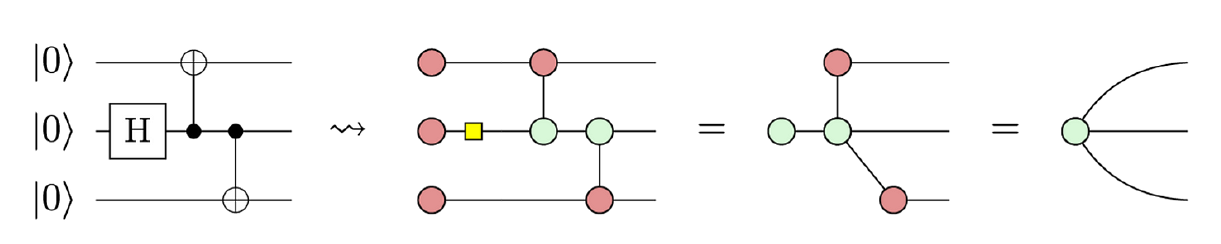
\includegraphics[width=0.5\textwidth]{images/ghz.png}
    \caption{GHZ Circuit}
    \label{fig:ghz}
\end{figure}

In order to achieve a simplification we will perform these steps:

\begin{enumerate}
    \item
          In the first step we translated the gates from the circuit into their corresponding ZX-diagrams. For this we used the \textbf{CNOT} and \textbf{Hadamard} rules from the previous section.
    \item
          Now we can start simplifying the diagram. We will start by applying the \textbf{Spider Fusion} rule to merge all free spiders together.
    \item
          Next we will apply the \textbf{Color Change} rule to change the color of the spider left of the Hadamard gate. This operation cancels out the Hadamard gate.
    \item
          After we perform the Spider Fusion rule again, and remove the identity spiders, we end up with the simplified diagram shown in rightmost diagram of figure \ref{fig:ghz}. Using the formula for calculating the matrix-representation of single spider we calculate $|GHZ\rangle = 1\cdot |000\rangle + 1\cdot |111\rangle = |000\rangle + |111\rangle$. Which is proportional to the real GHZ state. Remember that in order to get the real GHZ state we have to normalize the state first, which we did not do here.
\end{enumerate}

By using the intermediate steps of translating the circuit into a ZX-diagram first, we were able to effortlessly calculate the matrix-representation of the circuit. Which would have been a lot harder if we had to calculate the matrix-representation of the circuit using only its gates and the classical circuit model.

\subsection{Quantum Teleportation}

We will now look at a more complex example. We will look at the quantum teleportation circuit from figure \ref{fig:teleportation-classic}.



\begin{figure}[h]
    \centering
    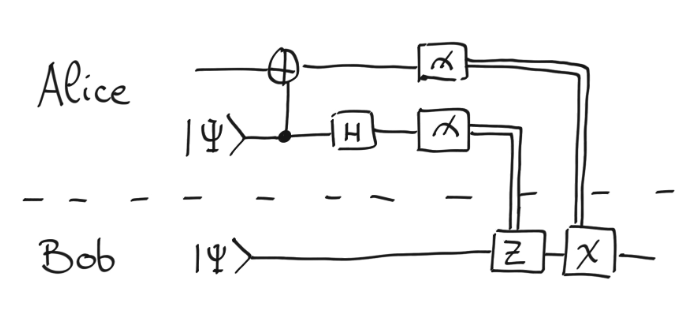
\includegraphics[width=0.45\textwidth]{images/teleportation-classic.png}
    \caption{Quantum Teleportation Circuit Img: Pennylane\cite{pennylane2023zx}}
    \label{fig:teleportation-classic}
\end{figure}

In order to understand the circuit we will first look at the representation of measurements in the ZX-Calculus. We will use the following rules to represent measurements in the ZX-Calculus. The measurements in the given basis are represented by parameterized spiders of the same basis \cite{vandewetering2020zxcalculus}. The parameter of the spider are boolean values, which represent the measurement outcome. Based on the outcome of the measurement we can influence other parts of the circuit, by including the parameter of the measurement spider in the target spiders of the other gates.

Another interesting thing to notice is that the shared bell state, which is the key to the quantum teleportation algorithm, can be represented by the spider
\zx{\zxNone{} \ar[d,C] \\[\zxWRow]    \zxNone{}} which has a matrix representation of $\begin{pmatrix}
        1 & 0 & 0 & 1 \\
    \end{pmatrix}^T$, and therefore is proportional to the bell state $|\phi^+\rangle$.


\begin{figure}[h]
    \centering
    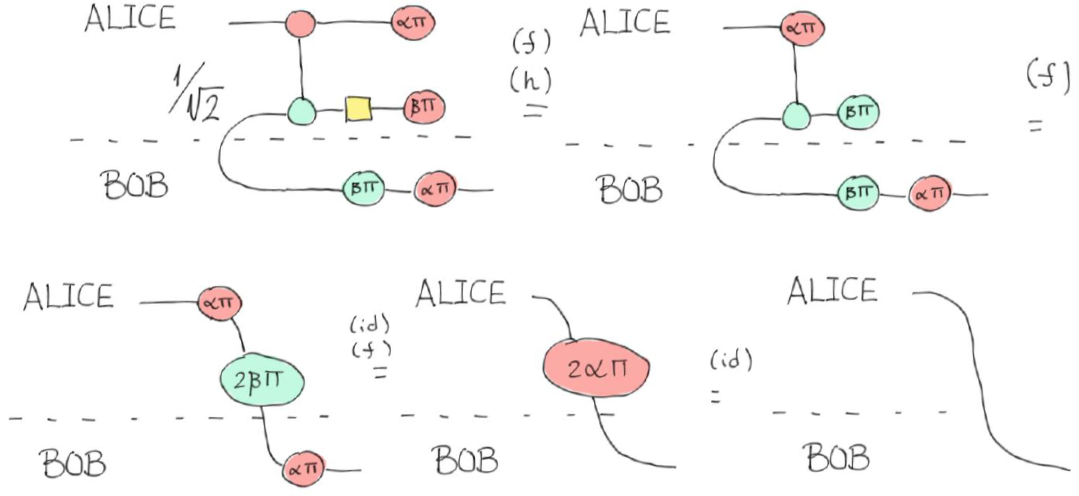
\includegraphics[width=0.45\textwidth]{images/teleportation.png}
    \caption{Teleportation in the ZX-Calculus Img: Pennylane\cite{pennylane2023zx}}
    \label{fig:teleportation}
\end{figure}

By applying the rewrite rules from above we can deduce that the whole circuit \textit{cancels} itself out. This means that the circuit is equivalent to the identity circuit between Alice and Bob. Therefore we showed that the teleportation works as expected.